% -----------------------------------------------------------------------------
% -- class
%\documentclass[titlepage,german,handout]{beamer}
\documentclass[titlepage,german,presentation]{beamer}
\usetheme{HUB}
\setbeamercovered{invisible}
\usepackage[noborder,colbullets]{beamerMACSYdefs}
% -----------------------------------------------------------------------------


% -----------------------------------------------------------------------------
% -- packages
\usepackage{babel}
\usepackage[utf8]{inputenc}
\usepackage[TS1,T1]{fontenc}
\usepackage{array}
\usepackage{multicol}
\usepackage[absolute,overlay]{textpos}
\usepackage{tikz}
\usepackage{colortbl}
\usepackage{amsmath}
\usepackage{amsthm}
\usepackage{amsfonts}
\usepackage{amssymb}
\usepackage{hyperref}
\usepackage{algorithm}
\usepackage{algorithmicx}
\usepackage{algpseudocode}
\usepackage{float}
\usepackage{graphicx}
\usepackage{caption}
\usepackage{subcaption}
% -----------------------------------------------------------------------------
\usepackage{multirow}

% -----------------------------------------------------------------------------
% -- custom commands
\input include/newcom
% \input include/macros

\newenvironment{rcases}{% 
  \left.\renewcommand*\lbrace.% 
  \begin{cases}}% 
{\end{cases}\right\rbrace}

\graphicspath{{./images/}}
\makeatletter
\renewcommand{\heading}[1]{\vspace{4.9\K@pt}\par{\KIT@fnt@hdr#1}\vspace{-0.25em}}
\makeatother
% -----------------------------------------------------------------------------


% -----------------------------------------------------------------------------
% -- titlepage
% -----------------------------------------------------------------------------

\title{Seminar on Graph Algorithms}
\subtitle{Streaming Graph Challenge: Stochastic Block Partition}


\author{Prof. Dr. Henning Meyerhenke, Dr. Maria Predari, Eugenio Angiman}
\institute{HU Berlin $\cdot$ Institut für Informatik $\cdot$ Modellierung und Analyse komplexer Systeme}

\TitleImage[height=\titleimageht]{images/title-networks}

\begin{document}
\setlength\textheight{7cm} %required for correct vertical alignment, if [t] is not used as documentclass parameter

\begin{frame}
 \maketitle
\end{frame}

\AtBeginSection[]
 {
 \begin{frame}
   \frametitle{Inhalt}
   \tableofcontents[currentsection]
 \end{frame}
 }
 % -----------------------------------------------------------------------------



% -----------------------------------------------------------------------------
% include of the respective lectures
%
%% -----------------------------------------------------------------------------
\begin{frame}{Herzlich Willkommen!}
%
\begin{itemize}
  \item \textbf{Vorlesung:} \\ Algorithmische Methoden für schwere Optimierungsprobleme
\medskip
  \item \textbf{Bereich:} Bachelor Informatik (und verwandt), \\ typischerweise 3. Jahr
\bigskip
  \item \textbf{Dozent:} Prof.\ Dr.\ Henning Meyerhenke
\medskip
  \item \textbf{Übungsleiter:} Dr. Alexander van der Grinten
\end{itemize}
%
\end{frame}
% -----------------------------------------------------------------------------


% -----------------------------------------------------------------------------
\begin{frame}{Begriffserklärungen}
%
\begin{itemize}
  \item Algorithmische Methoden
  \begin{itemize}
    \item Welche?
  \end{itemize}
\end{itemize}

\medskip
für
\medskip

\begin{itemize}
  \item schwere Optimierungsprobleme
  \begin{itemize}
    \item Was?
    \item Welche?
  \end{itemize}
\end{itemize}
%
\pause
\medskip
%
\textbf{Wozu?}
%
\end{frame}
% -----------------------------------------------------------------------------


%% Graph coloring
%\include{include/GF/vorl-01}
%\include{include/GF/vorl-02}
%\include{include/GF/vorl-03}
%\include{include/GF/vorl-04}

%% Bin packing
%\include{include/BP/vorl-01}
%\include{include/BP/vorl-02}
% \include{include/BP/vorl-03}
% \include{include/BP/vorl-04}

%% TSP
%\include{include/TSP/vorl-01}
%\include{include/TSP/vorl-02}
%\include{include/TSP/vorl-03}

%% SAT
%\include{include/SAT/vorl-01}
%\include{include/SAT/vorl-02}
%\include{include/SAT/vorl-03}

%\include{include/vorl-08}
%%\include{include/vorl-09}
%\include{include/vorl-10}
%%\include{include/vorl-11}
%%\include{include/vorl-12}
%\include{include/vorl-13}
%%\include{include/vorl-14}
%\include{include/vorl-15_roland}
%
% end include
% -----------------------------------------------------------------------------


% 


 \begin{frame}{Preliminary Discussion}

   \begin{center}
     \huge
   Welcome to the graph algorithm seminar!\\
   \end{center}

\begin{itemize}
\item General Organization
\item Communication and Evaluation
\item Schedule and Assignments
\item Presentation of Topics
\end{itemize}


\end{frame}

\begin{frame}
\frametitle{Graph Partitioning/Clustering Problem}

\begin{block}{Definition}
  Discover distrinct community structure in a graph
  such that nodes of the same community are more similar
  (in some sense) to each other than nodes of other
  communities
\end{block}

Applications in social networks, biology etc.\\

\begin{center}
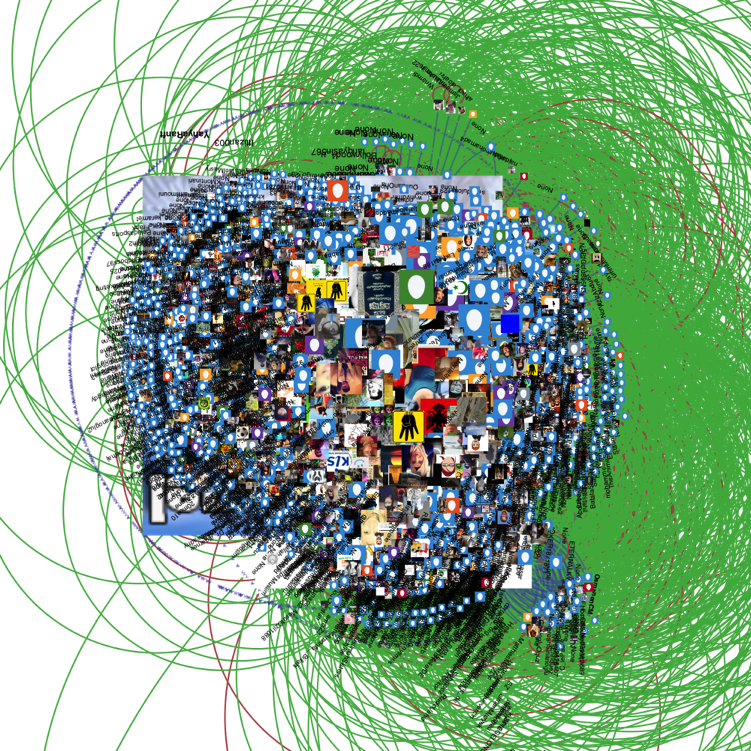
\includegraphics[height=0.22\textwidth]{./ch/1476395085.png}\qquad
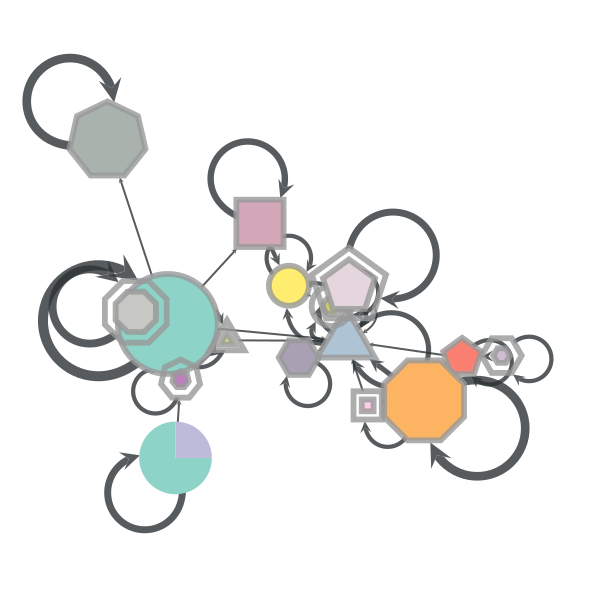
\includegraphics[height=0.22\textwidth]{./ch/1476395079.png}
~\\
social media network \qquad sub-network blocks
\end{center}

\end{frame}

\begin{frame}[allowframebreaks]
        \frametitle{References}
        %        \bibliographystyle{amsalpha}
        \bibliographystyle{acm}
        \bibliography{biblio}
\end{frame}



%% %%%%%%%%%%%%%%%%%%%%%%%%%%%%%%%%%%%%%%%%%
%% %%%%%%%%%%%%%%%%%%%%%%%%%%%%%%%%%%%%%%%%%
%% \begin{frame}
%% \frametitle{References (1)}

%% \begin{itemize}
%% \item[1.]
%% R.~{Diestel}.\\
%% {\em {Graph Theory}}, volume 173 of {\em Graduate Texts in Mathematics}.\\
%% Springer, 2010.

%% \item[2.]
%% J.~{Edmonds}.\\
%% Paths, trees, and flowers.\\
%% {\em Canad. J. Math.}, 17:449--467, 1965.

%% \item[3.]
%% J.~{Eisner}.\\
%% State-of-the-art algorithms for minimum spanning trees - a tutorial discussion, 1997.

%% \end{itemize}
%% \end{frame}

%% %%%%%%%%%%%%%%%%%%%%%%%%%%%%%%%%%%%%%%%%%
%% \begin{frame}
%% \frametitle{References (2)}

%% \begin{itemize}
%% \item[4.]
%% A.~V. {Goldberg} and C.~{Harrelson}.\\
%% Computing the shortest path: $A^*$ search meets graph theory.\\
%% In {\em Proceedings of the Sixteenth Annual ACM-SIAM Symposium on
%%   Discrete Algorithms}, SODA '05, pages 156--165, Philadelphia, PA, USA, 2005.
%%   %Society for Industrial and Applied Mathematics.

%% \item[5.]
%% P.~E. {Hart}, N.~J. {Nilsson}, and B.~{Raphael}.\\
%% A formal basis for the heuristic determination of minimum cost paths.\\
%% {\em IEEE Transactions on Systems, Science, and Cybernetics},
%%   SSC-4(2):100--107, 1968.
%% \end{itemize}

%% \end{frame}

%% %%%%%%%%%%%%%%%%%%%%%%%%%%%%%%%%%%%%%%%%%
%% \begin{frame}
%% \frametitle{References (3)}

%% \begin{itemize}
%% \item[6.]
%% D.~R. {Karger} and C.~{Stein}.\\
%% A new approach to the minimum cut problem.
%% {\em J. ACM}, 43(4):601--640, 1996.

%% \item[7.]
%% S.O. Krumke and H.~Noltemeier.\\
%% {\em Graphentheoretische Konzepte und Algorithmen}.\\
%% Leitf{\"a}den der Informatik. Vieweg + Teubner, 2009.

%% \item[8.]
%% J.~{Misra} and D.~{Gries}.\\
%% A constructive proof of Vizing’s theorem.\\
%% {\em Information Processing Letters}, 41, 1992. 

%% \item[9.]
%% J.G. {Oxley}.\\
%% {\em Matroid theory}.\\
%% Oxford University Press, New York, USA, 1992.
%% \end{itemize}

%% \end{frame}

%% \begin{frame}
%% \frametitle{References (4)}

%% \begin{itemize}

%% \item[10.]
%% M.~Fiedler.\\
%% {\em Algebraic connectivity of Graphs}.\\
%%  Czechoslovak Mathematical Journal 23(98) (1973), 298?305.

%% \item[11.]
%% R.~Lipton, and R.~Tarjan.\\
%% {\em A separator theorem for planar graphs}.\\
%% Siam J. Appl. Math., Vol. 36, No. 2, pages 177?189, 1979.

%% \item[12.]
%% Micha Sharir.\\
%% \em{ A strong connectivity algorithm and its applications to data flow analysis}.\\
%% Computers and Mathematics with Applications 7(1):67?72, 1981.
%% \end{itemize}

%% \end{frame}

%% \begin{frame}
%% \frametitle{References (5)}

%% \begin{itemize}

%% \item[13.]
%% Tarjan,~R.~E.\\  
%% {\em Depth-first search and linear graph algorithms}.\\
%% SIAM Journal on Computing, 1 (2): 146?160, 1972.

%% \item[14.]
%% Bichot, Charles-Edmond and Siarry, Patrick.\\
%% {\em Graph Partitioning: Optimisation and Applications}.\\
%% John Wiley \& Sons, 24 Jan 2013.
%% \vfill\clearpage
%% \end{itemize}

%% \end{frame}



\end{document}
